\subsubsection{\acrshort{lstm} layers}\label{lstm_theory}

The \acrfull{lstm} are the most used recurrent layers for its capacity to maintain long term dependencies and are widely used in deep learning communities.
\newline

The key behind \acrshort{lstm} are the gates that allow the neuron to actively add or remove information. It consists of several activation functions $\sigma$ and a $tanh$. The trigger function $\sigma$ results in the output value being a value between $0$ and $1$. Intuitively one can think of these functions as aiming to capture and retain information between $0$, or nothing, and $1$, everything.
\newline

Below is a diagram of how an \acrshort{lstm} gate works.

\begin{figure}[H]
    \centering
    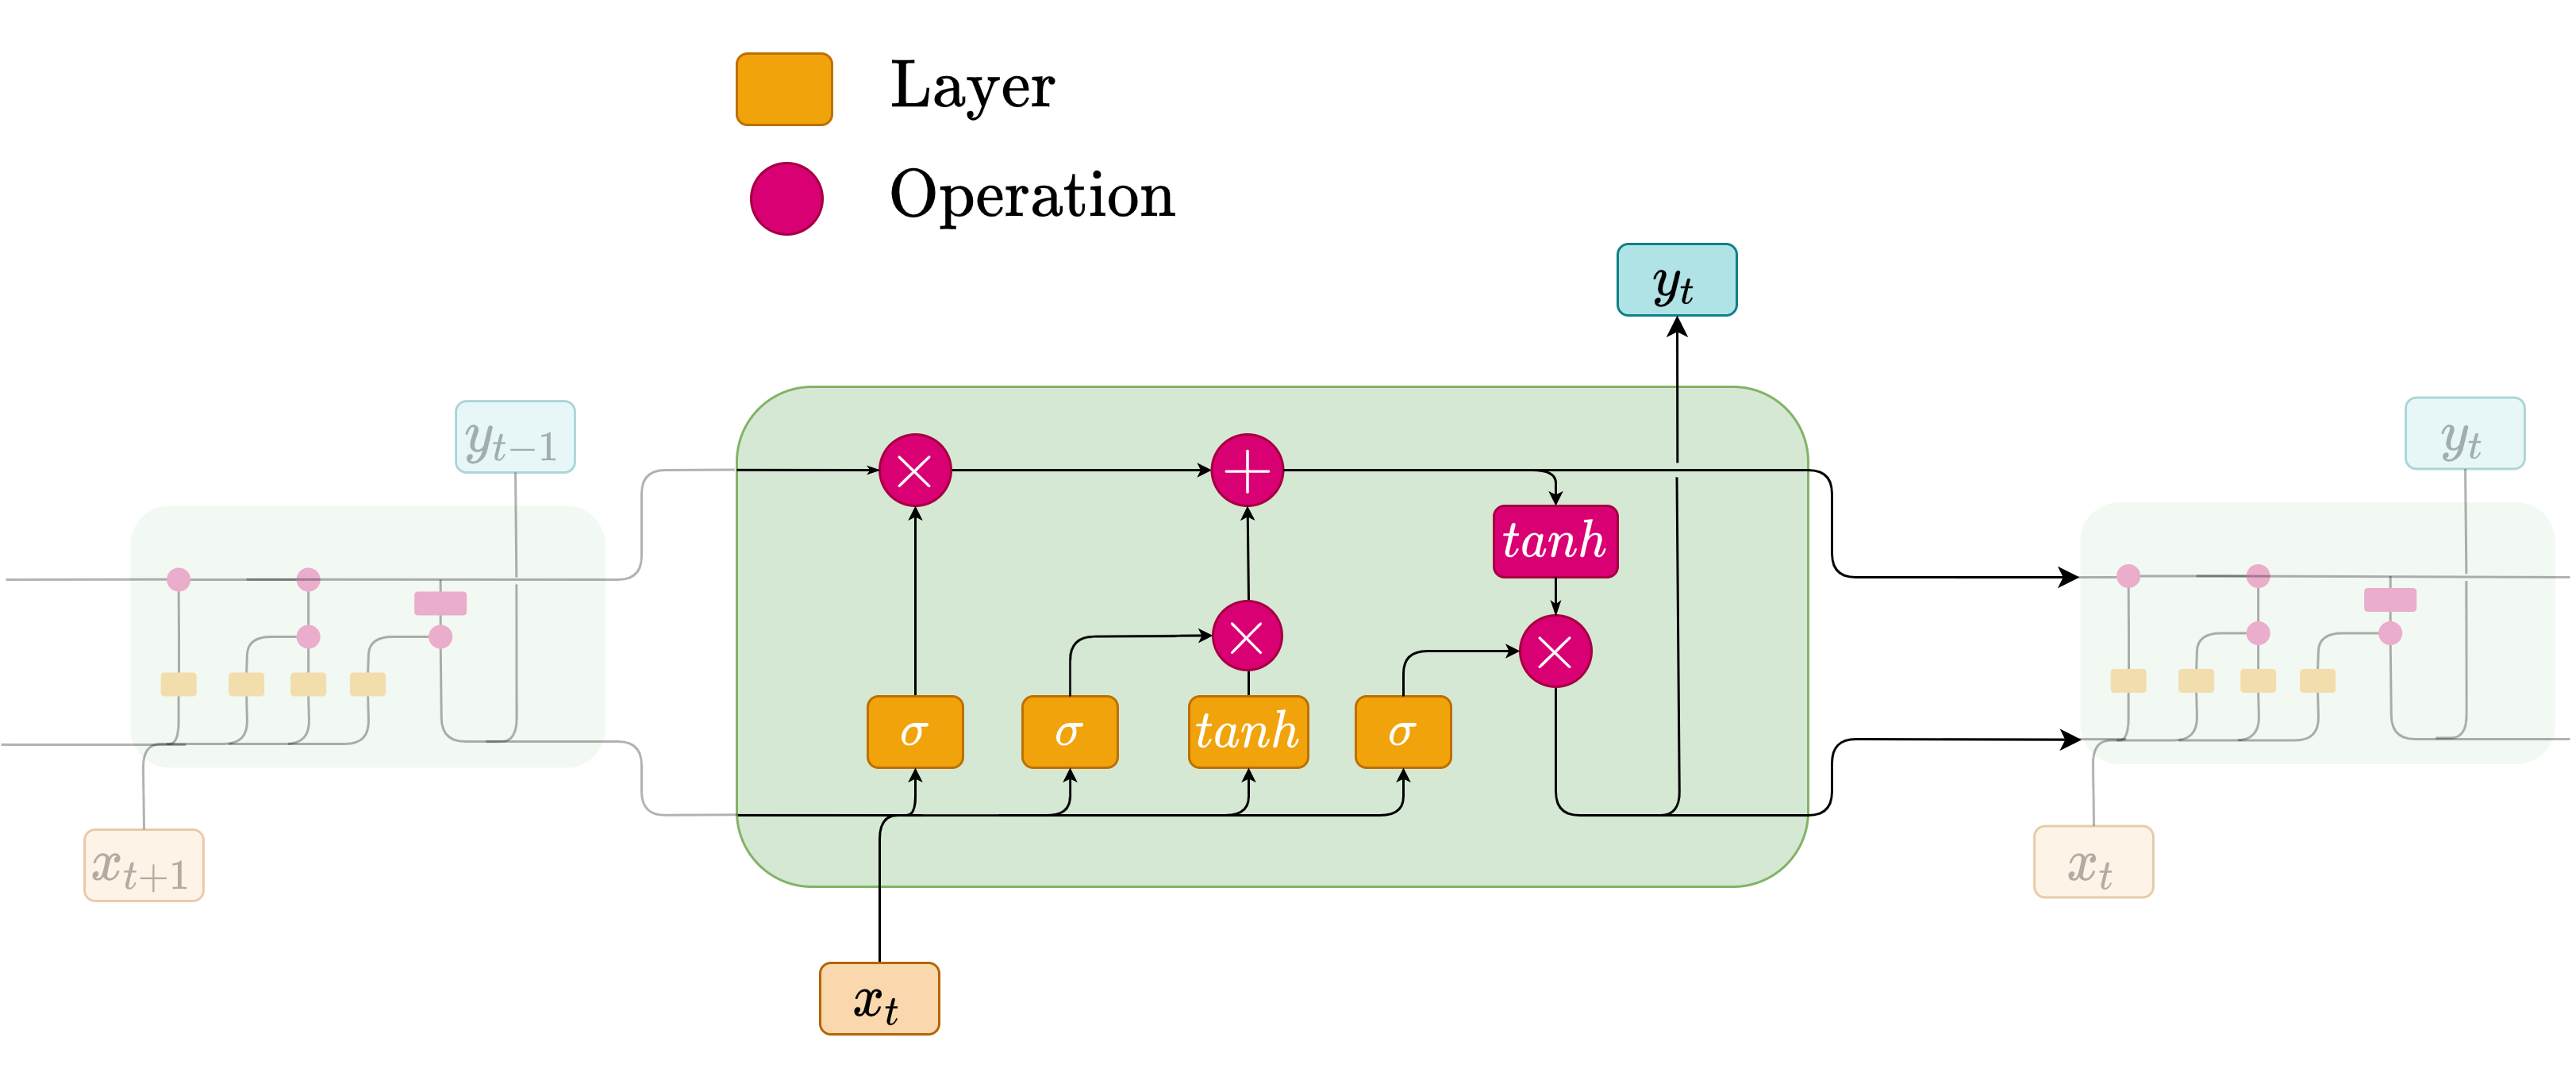
\includegraphics[width=16cm]{images/state-of-art/rnn/lstm.png}
    \caption{Behaviour of an \acrshort{lstm}}
\end{figure}


\acrshort{lstm}s are basically formed by four different steps:
\begin{enumerate}
    \item Forgetting irrelevant information: In the first output of this part is the first function $\sigma$ together with the operation of the product to scale between the output of $\sigma$ and the previous state $h_{t-1}$.
    \item Save new information: It consists of the second function $\sigma$ and the $tanh$ function next to it.
    \item Use the two previous steps to calculate a new internal state $h_t$: It is the part represented by the top line and calculate $c_t$. This vector is usually considered as the \acrshort{lstm} memory.
    \item Compute output value $y_t$: Formed by the last function $\sigma$ and by the $tanh$ function. It controls which information is important and saves the information about the current status.
\end{enumerate}

With this gate design, a recursive neuron can be designed to allow the flow of the gradients uninterruptedly and prevent them from fading.
\newline

%TODO LSTM GRADIENT FLWO
% https://youtu.be/SEnXr6v2ifU?list=PLtBw6njQRU-rwp5__7C0oIVt26ZgjG9NI&t=2109
 
 
 In summary, an \acrshort{lstm} neuron allows both memory and internal state to be separated into two parts allowing the network to learn long-term dependencies in one sequence. It does this by using gates to control the flow of information: forgetting irrelevant information, saving important information, selectively updating the internal state and saving part of the information. All this allowing the flow of the gradients to be unaltered to avoid the fading of the gradient.